\sectioncentered*{Введение}
\addcontentsline{toc}{section}{Введение}
\label{sec:intro}
Гиперспектральная съемка развивающиеся и перспективное направление дистанционного зондирования земной поверхности. В основе данного вида съемки лежит понятие гиперспектрального изображения. Гиперспектральное изображение -- это трехмерный массив данных, который хранит двухмерную информацию о пространственных координатах и дополнительные одномерные данные о спектральных характеристиках точки поверхности. Данная технология широко применяется в различных сферах, таких как:
\begin{itemize}
    \item сельское хозяйство;
    \item медицина;
    \item производство и переработка продуктов питания;
    \item минералогия;
    \item физика;
    \item астрономия;
    \item химическая визуализация.
\end{itemize}
Существует множество различных методов получения данного типа изображения, один из которых использует статический Фурье-спектрометр на основе интерферометра Саньяка. Данный метод налагает свои ограничения на данные получаемые во время съемки. Для построения гиперспектрального изображения требуется накопить достаточное количество данных о точке местности, в процессе ее прохождения вдоль направления полета. Ввиду того, что в дальнейшем над полученными сигналами выполняется дискретное преобразование Фурье, к ним предъявляются строгие требования. В частности необходимо чтобы полученный сигнал относился к одному и тому же участку местности, а его частота дискретизации была равномерной. В лабораторных и других стабильных условиях съемки, когда частоту кадров можно синхронизировать со скоростью полета, достаточно смещать каждый кадр на один пиксель. Таким образом легко получить информацию о яркости любого пикселя под разными углами съемки. При съемке с различных летательных аппаратов вибрации и колебания не позволяют использовать методы применяемые в камерах установленных на спутниках. Для сведения задачи к вышеописанному случаю требуется отдельно обработать получаемые при съемке местности данные. Для этого необходимо совместить соседние кадры и узнать их относительное перемещение. 

Основной задачей данной работы является реализация и анализ различных алгоритмов позволяющих решить вышеописанную проблему.

Предполагается, что использование детекторов границ позволит выделить особые участки изображений остающихся на соседних кадрах и отражающие взаимное смещение между ними. Тем самым сокращая перебор.  

\section{Описание среды разработки}
\label{sec:env_description}
В данном разделе будут рассмотрены различные инструменты используемые в ходе выполнения работы, их процесс установки и специфика использования. Также будет произведен краткий сравнительный анализ аналогичных средств, будет дано обоснование выбора именно тех средств, которые использованы в данной работе. 
\subsection{Visual Studio}
\label{sub:env_description:vs}
\textit{Microsoft Visual Studio} -- линейка продуктов компании Microsoft, включающих интегрированную среду разработки программного обеспечения и ряд других инструментальных средств. Данные продукты позволяют разрабатывать как консольные приложения, так и приложения с графическим интерфейсом, в том числе с поддержкой технологии Windows Forms, а также веб-сайты, веб-приложения, веб-службы как в родном, так и в управляемом кодах для всех платформ, поддерживаемых Windows, Windows Mobile, Windows CE, .NET Framework, Xbox, Windows Phone .NET Compact Framework и Silverlight.

Visual Studio является одним из лидеров среди интегрированных сред разработки на языке C++. Высокая популярность данной среды выражается в огромном мировом сообществе разработчиков использующих её. Благодаря этому у разработчика, применяющего Visual Studio для решения своих задач, появляется возможность более быстрого решения часто возникающих проблем. Также большинство сторонних библиотек и других инструментов имеют версию специально выпущенную для Visual Studio. Большой ассортимент плагинов и расширений доступен в официальном онлайн магазине Microsoft. Почти все они доступны бесплатно. Данные дополнения позволяют упростить разработку и интегрироваться со сторонними сервисами. В частности в ходе разработки данного проекта применялся плагин VisualSVN, обеспечивающий возможность работать с системой контроля версий SVN.

Visual Studio является коммерческим проектом, однако для некоммерческой разработки предоставляется специализированная версия Community. По сравнению с версией Professional данная версия обладает ограниченным функционалом, однако в работе этот функционал не использовался. Поэтому разработка велась на версии Visual Studio 2017 Community RC.

Для начала установки требуется скачать установщик с официального сайта Microsoft\footnote{\url{https://www.visualstudio.com/ru/downloads/}}. Там располагается ссылка для скачивания. Скачанный файл запустит процесс установки, предварительно попросив принять условия лицензионного соглашения. Для перехода на следующий этап требуется нажать кнопку \textit{<<Продолжить>>} . После этого запустится Visual Studio Installer, который служит для установки и модернизации различных версий Visual Studio 2017.


\begin{comment}
\begin{figure}
    \centering   
    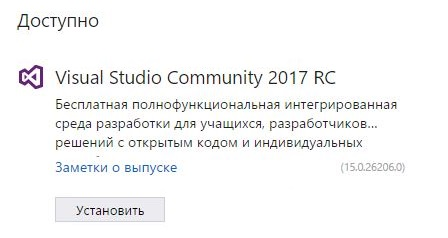
\includegraphics[width = 0.5\textwidth]{vs_install.JPG} 
    \caption{Выбор требуемой версии Visual Studio}
    \label{fig:vs_install2}
\end{figure}

\begin{figure}[h]
    \centering
    \begin{subfigure}{0.45\textwidth}  
        \centering     
        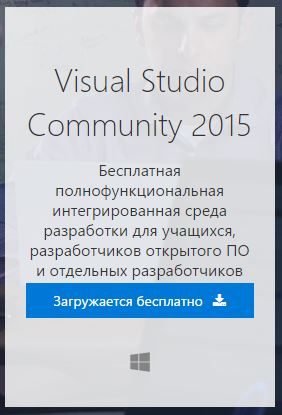
\includegraphics[width = \textwidth]{vs_download.JPG}
        \caption{}
        \label{fig:vs_downolad}
    \end{subfigure}
    \begin{subfigure}{0.45\textwidth}  
        \centering
        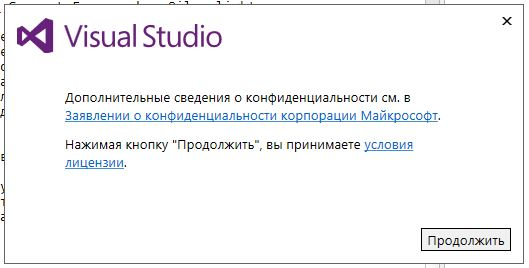
\includegraphics[width = \textwidth]{vs_licence.JPG}
        \caption{}
        \label{fig:vs_licence}
    \end{subfigure}
    \caption{а -- Ссылка для загрузки установщика; б -- окно принятия лицензионного соглашения}
    \label{fig:vs_install1}
\end{figure}
\end{comment}
После выбора нужной версии Visual Studio и нажатия кнопки \textit{<<Установить>>} откроется окно выбора комплектации среды разработки и дополнительных приложений, показное на рисунке \ref{fig:vs_install_chouse}. Для работы с данным проектом достаточно выбрать пункт \textit{<<Разработка классических приложений на C++>>} и предпочтительные языковые пакеты на вкладке \textit{<<Языковые пакеты>>}. Однако в зависимости от потребностей пользователя можно установить и дополнительные пакеты. Нажатие на кнопку \textit{<<Установить>>} запустит процесс установки Visual Studio.  После его завершения можно запустить среду разработки. При первом запуске запрашивается вход под аккаунтом Microsoft, если он еще не зарегистрирован то можно, или пропустить данный шаг и работать в неавторизированной версии, или зарегистрироваться на официальном сайте Microsoft.

\begin{figure}
    \centering   
    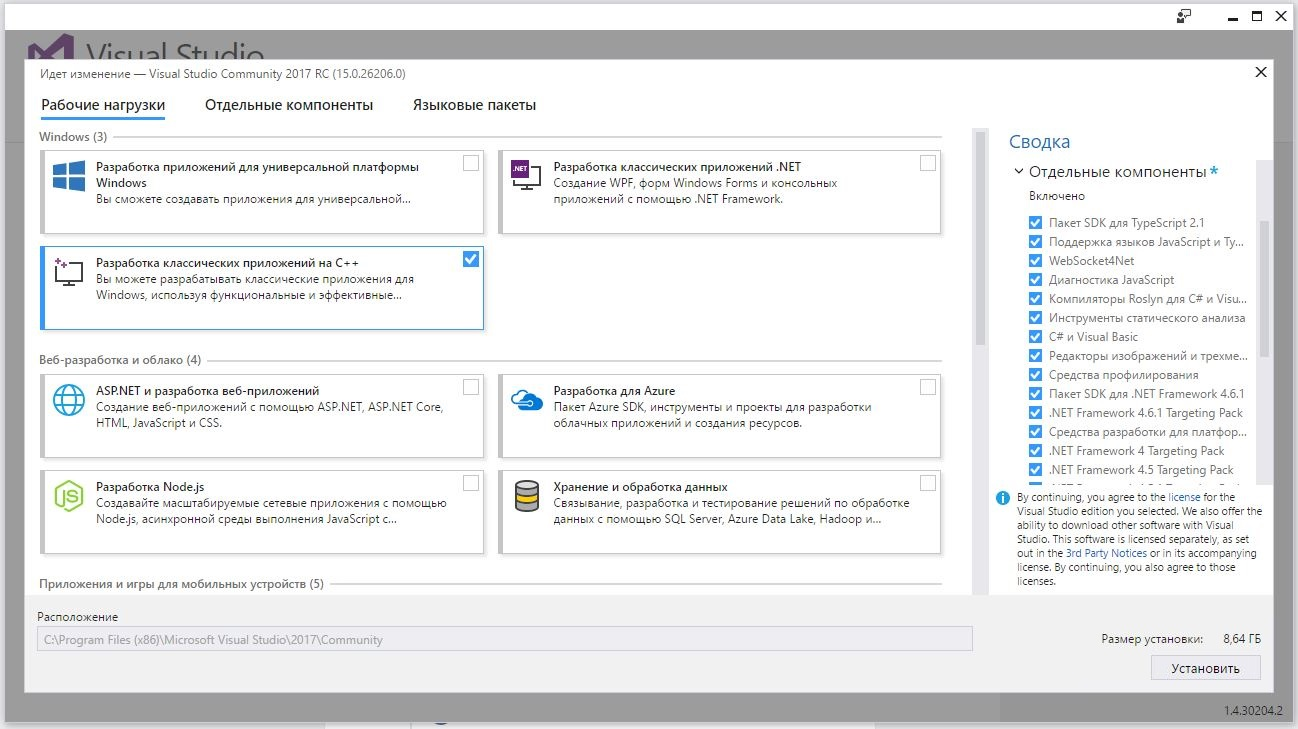
\includegraphics[width = \textwidth]{vs_install_chouse.JPG} 
    \caption{Окно выбора комплектации среды разработки и дополнительных приложений }
    \label{fig:vs_install_chouse}
\end{figure} 

\begin{comment}
\begin{figure}
    \centering   
    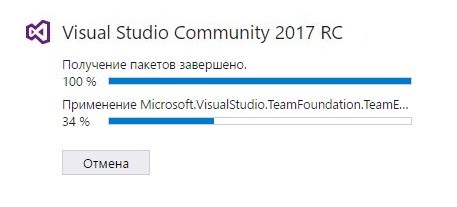
\includegraphics{vs_install2.JPG} 
    \caption{Процесс скачивания и установки Visual Studio}
    \label{fig:vs_install_progress}
\end{figure} 
\end{comment}
\subsection{OpenCV}
\label{sub:env_description:opencv}
\textit{OpenCV} -- выпущенная под лицензией BSD библиотека, а следовательно бесплатная для коммерческого и академического использования. Она имеет интерфейсы для C++, C, Python и Java. Поддерживает такие операционные системы как: Windows, Linux, Mac OS, Android и IOS. OpenCV была разработана для обеспечения эффективных вычислений с ориентацией на приложения реального времени. Написанная на оптимизированном C/C++, библиотека способна использовать преимущества многоядерной обработки. Работая вместе с OpenCL она может использовать возможности аппаратного ускорения. Используемая во всем мире, OpenCV насчитывает более 47 тысячи человек в сообществе пользователей и более девяти миллионов скачиваний. Применяется в различных сферах, начиная с интерактивного искусства, обнаружения мин или построения спутниковых карт до современной робототехники \cite{opencv_offical}.

\textit{OpenCV} -- наиболее полная, постоянно развивающаяся библиотека для обработки изображений. Огромное количество функций реализующих различные алгоритмы для обработки и анализа изображений позволяют сосредоточится на решении конкретной задачи, не отвлекаясь на написание заново уже известных классических алгоритмов. Наиболее сильным конкурентом OpenCV в сфере цифровой обработки изображений является MATLAB. Однако он больше подходит для прототипной разработки и исследований алгоритмов из-за удобства отладки, в скорости работы конечного приложения MATLAB сильно уступает возможностям OpenCV. Остальные аналоги реализуют ее функционал лишь частично и оптимизированы для определенной сферы применения Исходя из этих преимуществ OpenCV выбрана в качестве основного инструмента для разработки данного проекта. 

\section{Теоретический обзор используемых алгоритмов}
\label{sec:realization}
В целях анализа возможности применения детекторов границ для решения задачи совмещения изображения были отобраны три оператора. Основанием для отбора этих операторов послужила их простота реализации и скорость работы. Качество найденных границ не учитывалось, ввиду того, что нет необходимости в точности выделенных объектов, требуется только найти особые области сохраняющие свою форму, ориентацию между кадрами и свое положение относительно земной поверхности.

Все ниже описанные операторы используют различные матрицы для приближенного вычисления первой производной изображения, таким образом резкие границы изменения яркости легко обнаружить на основании того, что их первые производные превосходят по модулю некоторый порог.
\subsection{Оператор Робертса}
Один из старейших детекторов разработанный Л. Робертсом в 1963 году \cite{RobertsPhD}. По своей сути вычисляет сумму квадратов разниц между диагонально смежными пикселами. Это может быть выполнено сверткой изображения с двумя ядрами:

\begin{equation}
\begin{bmatrix}
+1 & 0\\
0 & -1
\end{bmatrix}
and
\begin{bmatrix}
0 & +1\\
-1 & 0
\end{bmatrix}
\end{equation}
\\
\subsection{Оператор Собеля}
Дискретный дифференциальный оператор, вычисляющий приближённое значение градиента яркости изображения. Результатом применения оператора Собеля в каждой точке изображения является либо вектор градиента яркости в этой точке, либо его норма \cite{Sobel_14}. 

Оператор выполняет свертку двумя ядрами $3 \times 3$ для вычисления приближённых значений производных по горизонтали и по вертикали. Пусть $\mathbf{A}$ -- исходное изображение, а $\mathbf{G}_x$ и $\mathbf{G}_y$ приближенные производные вычисляемые следующим образом:

\begin{equation}
\mathbf{G}_y =
\begin{bmatrix}
    -1 & -2 & -1\\
    0 & 0 & 0 \\
    1 & 2 & 1    
\end{bmatrix}
\ast \mathbf{A}
;\;
\mathbf{G}_x =
\begin{bmatrix}
    -1 & 0 & 1\\
    -2 & 0 & 2 \\
    -1 & 0 & 1 
\end{bmatrix}
\ast \mathbf{A}
\end{equation}
\\
Где $\ast$ обозначает двумерную операцию свертки.

Приближенное значение модуля градиента можно вычислить путем взятия квадратного корня из суммы квадратов соответствующих элементов ранее вычисленных матриц.

\begin{equation}
G = \sqrt{{G_x}^2 + {G_y}^2}
\end{equation}\\

Дополнительно оператор Собеля позволяет вычислить направление градиента:

\begin{equation}
\theta = \arctan \left( \frac{G_y}{G_x} \right)  
\end{equation}\\
\subsection{Оператор Превитта}
Оператор Превитта использует следующие маски для приближения частных производных:
\begin{equation}\label{eq:prewitt}
\mathbf{G}_y =
\begin{bmatrix}
-1 & -1 & -1\\
0 & 0 & 0 \\
1 & 1 & 1    
\end{bmatrix}
\ast \mathbf{A}
;\;
\mathbf{G}_x =
\begin{bmatrix}
-1 & 0 & 1\\
-1 & 0 & 1 \\
-1 & 0 & 1 
\end{bmatrix}
\ast \mathbf{A}
\end{equation}

Данные маски аналогичны оператору Собеля и отличаются только коэффициентом 2 при средних элементах. Данные изменения влияют на уровень сглаживания.
\section{Разработка программы}
\subsection{Функциональное проектирование лабораторного стенда}
Программа реализована с использованием методологий ООП, что позволило повысить коэффициент повторного использования кода и улучшить его читаемость. В результате разработанные классы могут быть использованы при дальнейших разработках программ схожей тематики. Как можно увидеть из рисунка \ref{fig:uml} программа состоит из пяти классов, один из которых абстрактный и один статический. 
\begin{figure}[h]
    \centering   
    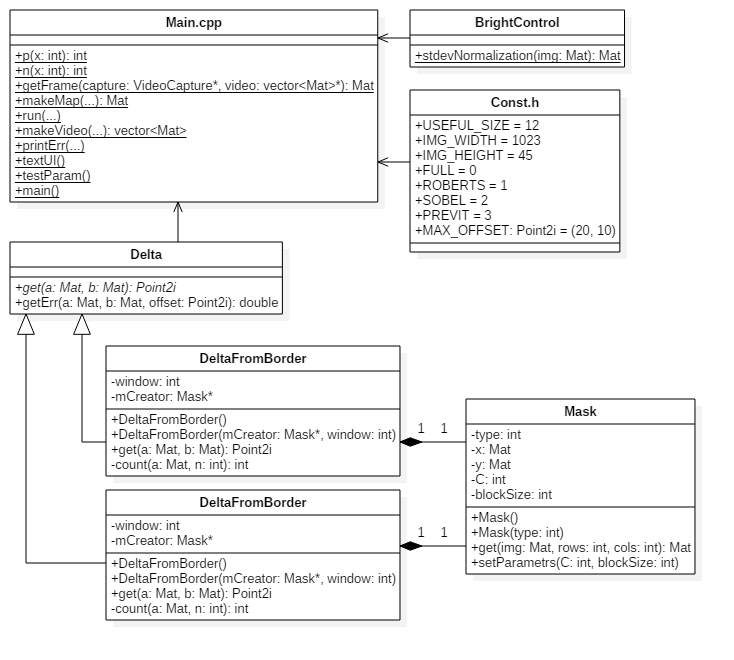
\includegraphics[width = \textwidth]{Main.png} 
    \caption{Структура программы}
    \label{fig:uml}
\end{figure} 

\subsubsection{Main.cpp~}
Содержит функции, реализующие основную логику программы и чтение/запись файлов. В некоторых из данных функций встречаются одинаковые параметры:

capture -- входной видеопоток из которого происходит чтение данных.

frameSize -- размер кадра оригинального видео.

video -- массив изображений в который покадрово записывается видео готовое к обработке.

offsets -- массив относительных смещений кадров, вычесляемых в процессе работы алгоритмов.

\texttt{main()} -- точка входа в программу. В зависимости от варианта сборки запускает функцию \texttt{textUI()} или \texttt{testParam()}.

\texttt{textUI()} -- реализует текстовый интерфейс для взаимодействия с пользователем. Как видно на рисунке \ref{fig:textUI} пользователь может выбрать тип маски и алгоритм, а также диапазон обрабатываемых кадров.
\begin{figure}[h]
    \centering   
    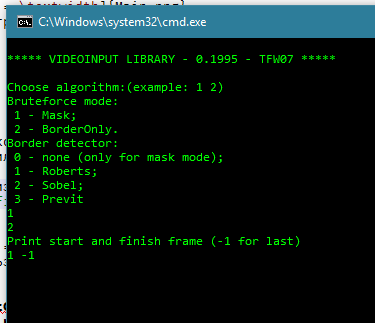
\includegraphics{textUI.png} 
    \caption{текстовый пользовательский интерфейс}
    \label{fig:textUI}
\end{figure} 

\texttt{testParam()} -- служит для многократного запуска алгоритма. Использование данной функции позволяет удобно тестировать алгоритмы при различных параметрах и собирать статистические данные. 

\texttt{vector<Mat> makeVideo( VideoCapture *capture, Size2i *frameSize, int start = 1, int length = -1)} -- загружает видео в виде вектора изображений из видео потока \texttt{capture}. Также возвращает размеры кадра. Может принимать номер первого кадра и длину получаемого видео. 

\texttt{Mat getFrame( VideoCapture *capture, vector<Mat> *video)} -- читает следующий кадр из видеопотока, подготавливает его и записывает в массив кадров.

\texttt{run( Size2i frameSize, vector<Mat> *video, Mat *map, Delta *delta,
    vector<Point2i> *offsets)} -- обрабатывает видео и запускает создание результирующего изображения \texttt{map}. Для этого принимает объект \texttt{delta} определяющий каким алгоритмом будет вычислено относительное смещение кадров.

\texttt{Mat makeMap( Size2i frameSize, vector<Mat> *video, vector<Point2i> *offsets,
    int maxL, int maxR, int maxD, int maxU)} -- создает результирующее изображение, для этого требуется узнать максимальные абсолютные смещения кадров во всех четырех направлениях.

\texttt{int printErr( vector<Mat> *video, vector<Point2i> *offsets, ofstream *sout, Mask *mCreator2)} -- выводит в текстовый файл дополнительные статистические данные.

\subsubsection{Класс BrightControl~}
Содержит единственный статический метод \texttt{Mat stdevNormalization(Mat img)} нормализующий изображение так, чтобы яркость любого пикселя подчинялась правилу трех сигм ($3\sigma$). Таким образом удается исправить резкие перепады яркости, мешающие работе основных алгоритмов. 
%TODO: вставить картинку демонстрирующую исправление пересвеченного кадра.
\subsubsection{Абстрактный класс Delta~}
Определяет интерфейс для работы с различными алгоритмами, которые вычисляют относительное смещение между соседними кадрами. Использование данного класса позволяет абстрагироваться от конкретной реализации, тем самым дает возможность использовать любой алгоритм без существенных изменений основного кода программы. 

Также включает дополнительную функцию \texttt{double getErr(Mat a, Mat b, Point2i offset)}. Она служит для вычисления ошибки совмещения изображений.
\subsubsection{Класс DeltaBruteForce~}
Реализует интерфейс \texttt{Delta}. Перебирает все возможные способы относительного смещения кадров, выбирая то, при котором средняя разница между соответствующими пикселями на кадрах будет минимальной. Учитывает только те пиксели, которые принадлежат области границ, для этого использует обнаруженные границы как маску.
\subsubsection{Класс DeltaFromBorder~}
Аналогично DeltaBruteForce реализует интерфейс \texttt{Delta} и перебирает все возможные способы относительного смещения кадров. Однако,  в этом случае выбирается то при котором область пересечения границ соответствующих кадров максимальна.
\subsubsection{Класс Mask~}
Выделяет границы на заданном изображении различными методами, возможно выбирать требуемый метод и параметры пороговой обработки.
\subsubsection{Const.h~}
Заголовочный файл содержащий некоторые константы упрощающие разработку и читаемость кода. Определяет константу \texttt{DF} позволяющую удобно создавать отладочную версию программы.
\section{Анализ полученных результатов}
В ходе разработки и тестирования возникала необходимость в исследовании и анализе некоторых параметров. 
\subsection{Максимальная амплитуда колебаний камеры}
На начальных этапах разработки потребовалось грубо оценить пределы колебаний камеры во время съемки, чтобы существенно сократит количество перебираемых вариантов в вышеописанных алгоритмах перебора.

Для этого было решено использовать метод щелевой съемки для визуального анализа скорости движения кадра по двум осям.

В отличии от обычной фотографии, которая запечатлевает определенный момент времени, щелевая позволяет наблюдать определенное узкое место (щель) на протяжении длительного момента времени. Принцип  формирования такого снимка изображен на рисунке \ref{img:splitGraph}.

В ходе исследования были созданы щелевые снимки для каждой из пространственной оси кадра, изображенные на рисунках \ref{img:splitX} и \ref{img:splitY}. Здесь красным и зеленым цветом выделены наиболее яркие и темные пиксели каждого кадра, для большего удобства визуального анализа.

По итогом исследования было установлено, что 
\subsection{Нахождение части кадра пригодной для обработки}
Как видно из рисунка \ref{img:semple} кадры получаемые со спектрометра имеют свою специфику, в частности можно выделить:
\begin{itemize}
	\item особый размер кадра, сильно вытянутый в ширину;
	\item интерференционные полосы в центре кадра. 
\end{itemize}
Для преодоления данных проблем потребовалось дополнительное исследование.

Широко известно, что оператор Робертса слабо чувствителен к вертикальным и горизонтальным границам. Поэтому была выдвинута гипотеза, что использование данного оператора позволит избежать влияния интерференционных полос. Однако, в ходе исследования, данная гипотеза не подтвердилась, что можно увидеть из рисунка \ref{fig:robertsComp}.

Так избежать влияния интерференции не удалось, то было принято решение выбрать часть кадра не подверженного данным помехам. В ходе визуального анализа было установлено, что верхняя или нижняя полоска кадра шириной в 12 пикселей свободна от сильных периодических шумов и достаточна для совмещения кадров между собой. 
\subsection{Параметры порогового фильтра}
На начальных этапах рассматривался вариант использования статического порогового фильтра, однако после серии экспериментов было установлено, что данный вид фильтра не обеспечивает стабильную плотность маски на разных участках съемки. Поэтому в дальнейшем исследовании использовался только адаптивный фильтр.

В пороговом фильтре существуют две свободные переменные, влияющие на качество результата: константа $C$ и размер окна. Для исследования влияния данных параметров на результат используются функции \texttt{testParam()} и \texttt{printErr()} в связке с дополнительной программой написанной на языке MATLAB. На рисунке \ref{fig:filterParamGraph} изображены графики показывающие зависимость средней ошибки совмещения от вышеуказанных параметров порогового фильтра для различных алгоритмов выделения границ.
